\documentclass{article}
\usepackage[margin=1.2in]{geometry}
\usepackage[utf8]{inputenc}
\usepackage{xcolor}
\usepackage{listings}
\usepackage{minted}
\usepackage{url}
\usepackage{graphicx}
\usepackage{epstopdf}
%\usepackage{caption}
%\usepackage[format=plain,margin=1.2in,labelfont=bf,up,textfont=it,up]{caption}
\usepackage[format=plain,margin=1.2in,labelfont=bf,up]{caption}
\captionsetup[figure]{font=footnotesize}
\usepackage{listings}
\usepackage{minted}
\usepackage{hyperref}

\begin{document}
\title{Learning-based semantic reconstruction in binary code}
\date{}
\maketitle

\abstract{In spite of significant advances in the field of binary program analysis over the last decade, the low-level of semantics present in binary code keeps challenging the accuracy and scalability of state-of-the-art models. Of particular interest is the problem of recovering accurate data-flow information from binary code, which is key to many security applications, but unfortunately remains a bottleneck in the context of many applications. The large semantic gap between high-level representations exhibited in source-code, and low-level binary code make it a challenge to apply well-known code analysis techniques, such as those used by compilers. 
	In this project, we aim to bridge the large semantic gap between source-level and binary-level representations by combining state-of-the-art binary program analysis techniques augmented with machine learning. Our primary focus is to improve the accuracy and scalability of data-flow analysis on binary code by reconstructing type semantics.
}

\section{Introduction and definitions}
The code executed by CPUs is expressed in binary form, whereas the code written by humans is mostly written in higher-level languages such as C or C++. A so-called ``executable'' program (\textit{e.g.,} exe on Windows, ELF on Linux and other UNIXes) is in binary form, and therefore qualifies as \emph{binary program}. Source code written by humans is translated into binary by a compiler (\textit{e.g.,} CLANG). Sometimes, expert humans write code in assembly language, a representation which is much closer to binary (or ``machine'') code. The process of transforming assembly code into binary code is done by an \emph{assembler}. The inverse process, \textit{i.e.,} going from binary to assembly is called \emph{disassembly}. The latter can also be applied to binaries that have been compiled from source. Disassembly is an essential process in reverse engineering, and is generally the first step in binary program analysis. However, because of discrepancies between processor architectures, there exists many different assembly languages (\textit{e.g.,} ARM, MIPS, X86, etc\ldots). While some binary analysis frameworks only support specific architectures, most  recent models and implementations \emph{lift} binary code into an architecture-agnostic representation called \emph{Intermediate Representation (IR)}.
Figure~\ref{fig:compilation} illustrates, from a high level, the processes of compilation (with CLANG) and reverse engineering (with angr). When compiling source-code, compilers generally employ an IR which allows them to perform most program analysis tasks in a generic way, regardless of the target architecture. Similarly, modern binary analysis platforms will lift binary code into an IR in order to abstract models and techniques away from the specificities of a single CPU architecture.

\subsection{Differences between IRs}
There exists, however, a key difference between the IR produced by a compiler and the IR produced by a disassembler: the compiler extracts meta-information from source code, such as types, variables and function names, which are kept in the intermediate stages of compilation. As a result, IRs used in compilers embed such meta-information, and only discard it in the final binary (executable) program representation.
Conversely, the IR produced by disassemblers is poor, and only reflects the information present in binary.

Remember that the first step in binary program analysis is generally to \emph{disassemble} binary code. Remaining analysis stages are generally performed at the IR level. Therefore, when we speak about binary analysis, we generally speak about the process of analyzing the lifted IR instead of directly analyzing the binary code. While this is conceptually equivalent, it is syntactically different.

Because of the large semantic gap between ``poor'' IR extracted from binary and the actual original source-code of a program, it is extremely difficult to recover the latter from the former (as indicated in red in Figure~\ref{fig:compilation}).

	\begin{figure}[h]
		\centering
		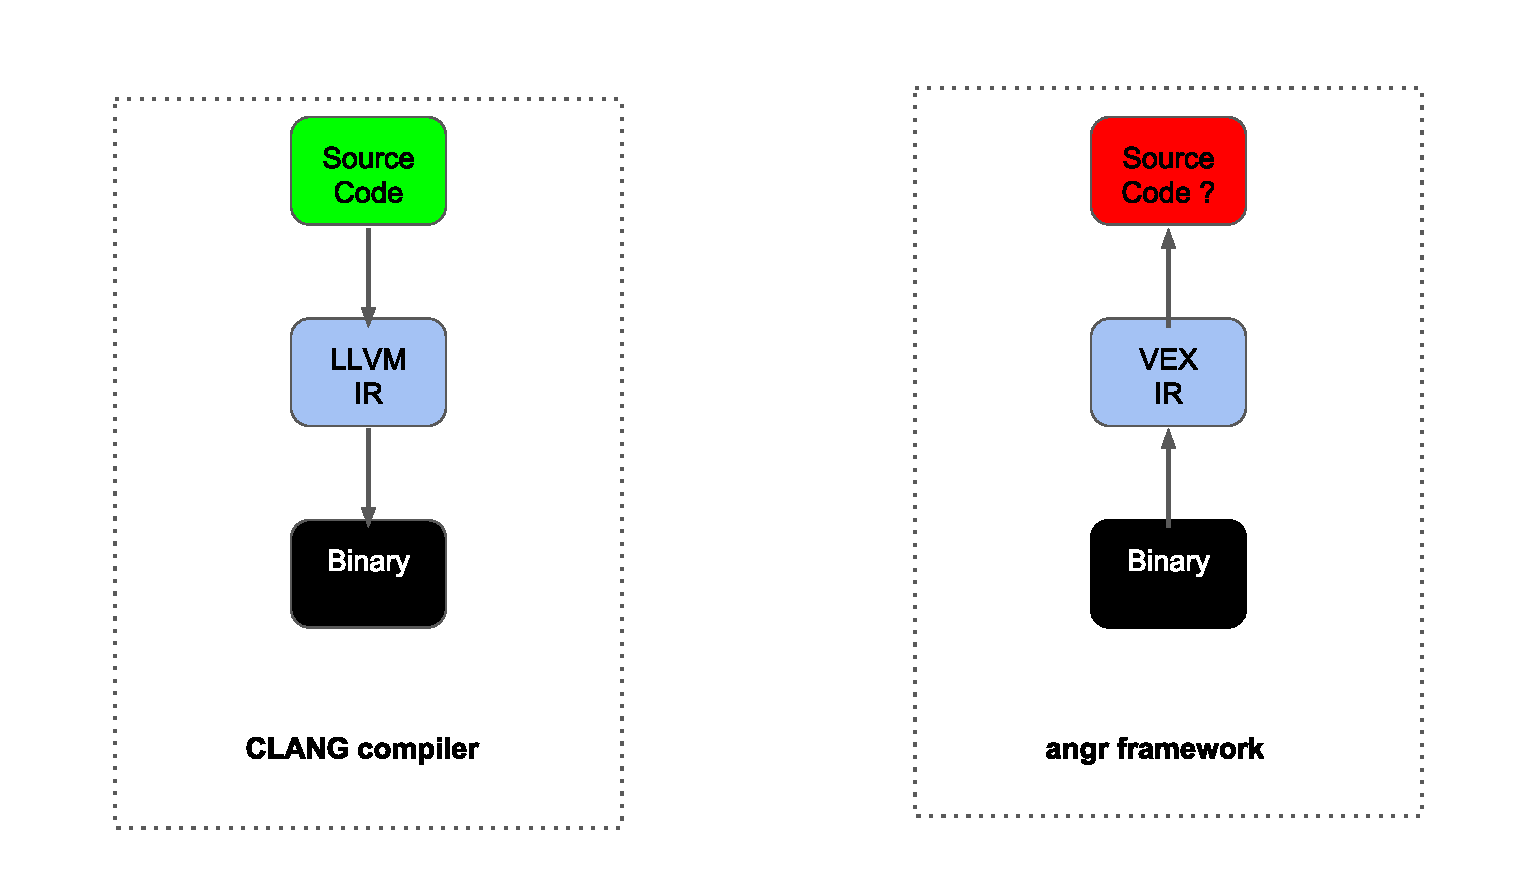
\includegraphics[width=.9\textwidth]{compilation.eps}
		\caption{Compilation with CLANG and binary analysis with \texttt{angr}. \texttt{angr} is a binary analysis platform built on top of the VEX intermediate representation.}
		\label{fig:compilation}
	\end{figure}

\subsection{Debug symbols}
Debugging is the process of identifying and removing errors from programs. In order for humans to relate low-level artifacts of a program (such as memory locations and registers) to high-level artifacts such as variables, functions and their associated names from the source code, it is possible to compile programs with so-called \emph{debug symbols}. These effectively provide a mapping between representations, which greatly eases the process of manually debugging programs.
The process of removing all debug information from a binary is called \emph{stripping}, and it is done by default when distributing software (which both saves space and makes reverse-engineering difficult).
In this project, we will use debug information as \emph{ground-truth} for learning purposes. We will work with ELF\footnote{\url{https://refspecs.linuxfoundation.org}} binaries on Linux, which support the DWARF\footnote{\url{http://dwarfstd.org}} representation for debug symbols.

\subsection{Execution}
When a program is executed, a component of the operating system called the \emph{loader} maps the binary program into memory. The original program file typically contains two segments: code and data. Code contains the actual program instructions, while data containts global variables as well as static variables. At runtime, the loader maps those segments into memory at different addresses. In addition, it creates two additional memory regions: the \emph{stack} and the \emph{heap}. The stack stores function arguments, local variables and return addresses, while the heap corresponds to dynamic memory allocation (\textit{i.e.,} \texttt{malloc()} and \texttt{free()}).

\section{Objectives}
Our primary objective is to recover information about \emph{types} in stripped binary code. At any point in the program, we would like to be able to tell whether the data that a given instruction manipulates is an \texttt{int} or a \texttt{char*} or a \texttt{struct XMLNode} from \texttt{libXML}. Composite types such as the latter are especially important, as these provide rich and important information about their inner members, as shown in Figure~\ref{fig:xmlnode}, such as function prototypes, and types of their inner fields, which are key to precise data-flow analysis.

\begin{figure}[!h]
	\centering
	\inputminted[xleftmargin=.1\linewidth, fontsize=\footnotesize, linenos, framesep=2mm, breaklines]{C}{xmlnode.h}
	\caption{Example of complex C structure as found in \texttt{libXML}.}
	\label{fig:xmlnode}
\end{figure}

\subsection{Method and representations}

From the analysis of low-level artifacts of binary code, we aim to infer information about data structures, along with high-level artifacts which are not present in binary. Possible low-level artifacts are memory accesses, CPU instructions, and other constructs present in assembly, whereas high-level artifacts are high-level notions such as present in source-code, like types (\texttt{int}, \texttt{string}, \texttt{array}, \texttt{struct XMLNode}, or functional descriptions (e.g. ``function storing user input in an array'', or ``function computing a SHA1 hash'').


We will use the \texttt{angr} framework in order to manipulate and analyze low-level constructs from binary programs. \texttt{angr} uses the VEX IR, see \url{https://docs.angr.io/advanced-topics/ir} for more information.

\subsection{Variable recovery}
Variable recovery is the process of recovering variables, \textit{i.e.,} how the program's data layout looks like in memory, and what is the semantic of data. Without any clues about where data starts and ends, and what are the types of memory locations, the entire program data segment just looks like a gigantic slab of binary data: low-level representations offer no meta-data about program variables\footnote{With a few rare exceptions, such as relocated globals.}. In order to understand what is the data and its layout in memory, it is necessary to look at the code. 
Recovering variables is typically a two-step process, where memory access patterns are first identified in order to identify variable boundaries. Then, a second stage of analysis attempts to attribute type information based on artifacts of program semantics. 

\textbf{Static vs dynamic analysis} -- 
Dynamic analysis consists in first executing programs \emph{concretely} (\textit{i.e.,} real execution) before observing program behavior on so-called execution traces, each corresponding to one particular path throught the program given a set of (concrete) inputs.
Static analysis consists in simulating all the possible outcomes of executing a program.

When it comes to data structure recovery, dynamic analysis offers an accurate view of memory accesses, but within a scope limited to observable program paths. Conversely, static analysis offers a broad view of possible executions, but with limited accuracy in terms of memory accesses. This lack of accuray is the source of limitations when attempting to detect the boundaries of data strucutres such as composite types such as those denoted by the \texttt{struct} keyword, or arrays.

Examples of static and dynamic approaches in the literature include ASI~\cite{asi}, a static model based on Value Set Analysis (VSA)\footnote{An approach of static analysis through abstract interpretation which goal is to approximate the machine state at every instruction.}, and Howard~\cite{howard}, which is based on dynamic analysis following semantic rules, augmented with type information propagation (borrowed from ASI).

\textbf{Rule-based and learning-based models}
While ASI and Howard are based on semantic models, other approaches such as Laika~\cite{laika} and Debin~\cite{debin} employ learning to recover variables from binary.

Howard~\cite{howard} is based on semantic rules, while Laika~\cite{laika} attempts to recover data structures and their instantiations based on unspervized Bayesian learning on top of dynamic pointer analysis. Debin~\cite{debin} is a static approach which learns the mapping from program variables to their locations in the assembly code as registers and memory offsets, and then trains a classifier from millions of registers and memory offsets that are labeled whether they represent variables. Then, this classifier is used to recover source-level variables from low-level registers and memory offsets.

\subsection{Limitations of current approaches}
\begin{itemize}
	\item Lack of structure/object field sensitivity.
	\item ASI too inaccurate, Howard rule-based, Laika too Naive.
	\item Debin is most recent and performant but focusses on name recovery and
		-- Exampe of issues: jointly predicting memory offset and type is akin
		to saying "variables at ebp-10 are more likely to be called x or be
		typed int". (Note: Debin's joint model is not unlike code similarity recognition mechanisms) -- Can we focus the model on a restricted set of intuitively more reliable features? -- Drop names, focus on types -- Add struct field sensitivity -- Focus on improving data-flow analysis (def-use chains)
\end{itemize}

\subsection{Next steps}

\begin{itemize}
	\item Learning on top of a static rule-based model.
	\item Example about features to identify types for e.g., signed/unsigned/FP.
	\item Static vs dynamic and learning-based vs rule-based. What we want is learning-based to detect known data-structures form libraries (which is akin to code similarity), but also to generalize this behavior so that we can detect internal variables as well, with a focus on types (and not necessarily names, except for known data-structures) and with object-field sensitivity.
\end{itemize}

\bibliographystyle{plain}
\bibliography{description}

\end{document}
